\section{Results}

\subsection{Changing neuron parameters} 

As Potjans and Diesmann suggested (2014), neuron parameters do not play a big role in shaping the network behavior. This obviously doesn't mean that neurons don't play a fundamental role in the simulation, but it could hint that their approximation is already good enough to provide plausible results. 

In fact, in almost 40000 episodes the agent's best result was $\approx 2.20$ mean absolute error. Although it is an improvement of the original model, where the error was $\approx 9.26$, it is yet relatively far from the biological data.

Nevertheless, we have to consider that the agent was able to change the parameters for all neurons at once, differentiating only between excitatory and inhibitory populations. The $k$ factor dividing the actions was 20 during the first run, but the results looked capped at low values, so it was lowered to 5 in a subsequent run, to leave the agent a wider range of action.

\subsection{Changing synapses parameters} 

Synapses parameters control the amplitude of postsynaptic potential, the delays of the connections and the relative strength of inhibitory synaptic connections. Potjans and Diesmann (2014) called this value $g$ and they imposed $g = 4$, to reproduce the dynamics exhibited by the random balanced network through the dominance of inhibitory connection over the excitatory ones.

In this setup the agent found that the value of $g$ that optimized the output was $\approx 4.4$, which is a further step in the direction of strong inhibitory synapses. Moreover, analyzing the data from the training steps, a it is shown a negative correlation between error magnitude and the mean delay of inhibitory connections, while when the delay of excitatory connections increased, the error shrank. Still, the parameter that looked more influential was the $g$ value, while the one with lowest correlation with the reward was the standard deviation of the amplitude of excitatory post-synaptic potentials. 

Synapses parameters' optimization was only slightly more effective than neuron's, with an $\approx 1.96$ mean absolute error with $k = 5$. This probably was because considered synapses parameters, as neuron's, mostly regarded universal thresholds. Beside that, synapse parameters was only 6, against the 26 of neurons and 64 of structure. That certainly reduced the power of the agent on the simulated brain column.

One possibility at this time could be to reduce the $k$ factor to let the agent have wider actions, but,  the best results weren't achieved by extreme actions, so it wouldn't have been meaningful to do that.

\subsection{Changing structure parameters} 

The scenario where the model was trained to change the structure parameters was the most successful between the first three, and it achieved an absolute error of $\approx 0.031$ in around 40000 episodes. 

Every action was divided by a factor of 20, to restrict the action range. That was necessary considered that the structure parameters were 64 values, making the problem highly complex to solve.
\begin{table}[htbp]
	\begin{center} \vspace{5pt} \setlength{\arrayrulewidth}{0.3mm}
			\begin{tabular}{|c | c c c c|} 
				\hline
                         & Layer 2/3 & Layer 4 & Layer 5 & Layer 6 \\ [0.5ex]
				\hline
				Baseline & 0.751     & 4.29    & 6.816   & 1.126   \\
				\hline
				Results  & 0.29      & 1.40    & 2.52    & 0.50    \\
				\hline
				Target   & 0.30      & 1.40    & 2.50    & 0.50    \\
				\hline
			\end{tabular}
		\caption{Comparison between models}
	\end{center}
\end{table}
\\ The model was tested every 200 episodes without noise to monitor its learning curve. As you can see in the picture \ref{fig:structure}, after the first 20000 episodes the model converges slowly almost to the 0.
\begin{figure}[htbp]
	\centering
	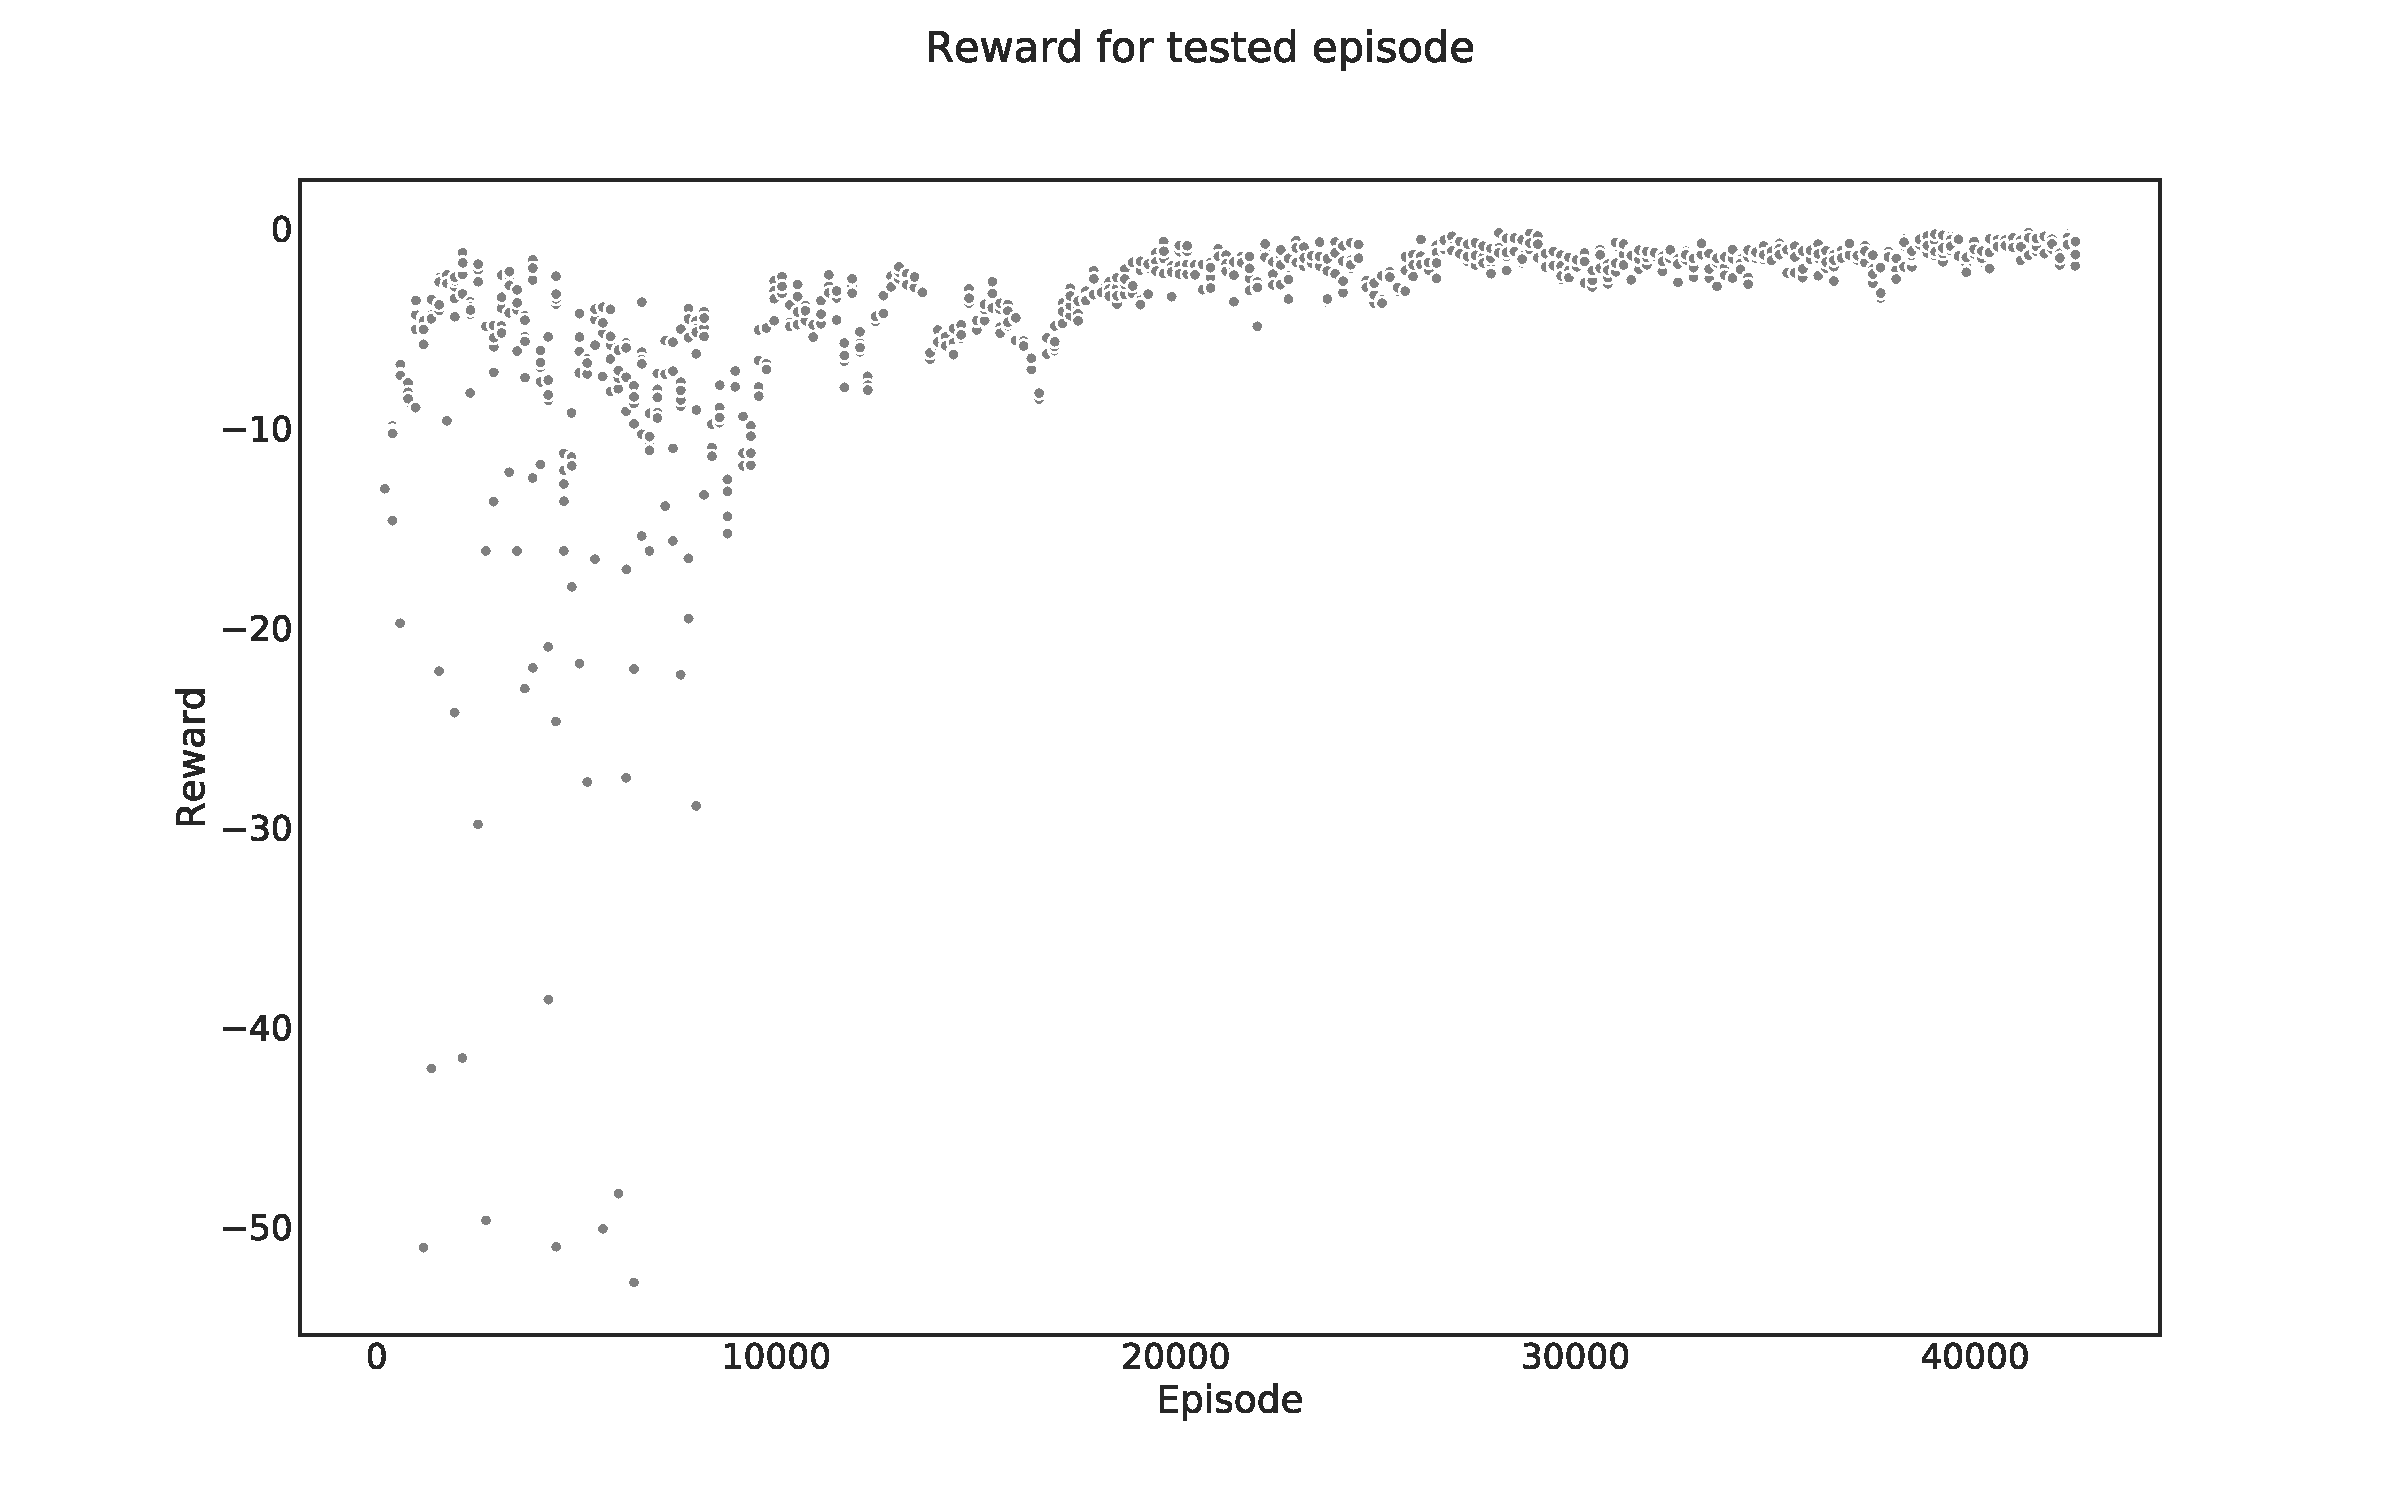
\includegraphics[scale=0.4]{pictures/structure_scatterplot.pdf}
	\caption{Absolute sum of errors}
	\label{fig:structure}
\end{figure}

\subsection{Changing all parameters} 
Interestingly, this case did not reach the results of the structure's scenario, only by less then $\approx 0.01$ absolute error, but to real difference was in the actions that it took to reach that error: while in the ``pure'' model the actions' absolute values were relatively small, in this case almost every action was at his limit, -1 or 1.

A possible interpretation can be that changing the synapses', neurons' and structure's parameters altogether, the agent actually optimizes the structure's parameters in a non-optimal state of the other parameters. In this case the agent would only need more training time, to be able to explore a larger share of its action space. 

